\chapter{Introduction}%    \chapter{}  = level 1, top level
	Imaging a place where thousands of boxes called containers flow through daily, carried by cranes or ships berth,
	orchestrating each movement to finally place them in a well-organized pile, set to be handled, rehandled,
	built, and retrieved when the time comes, to leave the port. For this logistical marvel, there is a critical
	challenge in this process: predicting, with precision, how long each box will stay to ensure they are moved only
	when necessary for their onward journey rather than to accommodate other cargo. This predictive capability can
	streamline port operations to reduce unnecessary movements while optimizing space utilization. This puzzle of
	time for improving movement and placements is the main point of this dissertation's inquiry.
	\\
	\\
	In today's fast-paced world of global trade, container ports are like the beating hearts of our supply chains.
	However, here is the thing: these ports face a constant puzzle – how to manage their limited space most
	efficiently. This is not about squeezing in as many containers as possible but knowing which ones will leave
	soon or stick around for a while.
	\\
	\\
	This research project was born from a collaboration with the Port of Auckland to find a way to use the data to
	optimize yard operations somehow. Following that mandate, using statistics, historical data, and the container’s
	movements and features, this project proposed building predictive models to predict dwell times
	\cite{merckx2005issue}
	, implementing machine learning techniques that can be involved inside the decision support system DSS (
	Figure~\ref{fig:dds_architecture}
	) to help day-to-day operations by making decisions based on predicting plausible days of container stays.
	\\
	\\
	That is where this research comes in to develop a machine learning model for doing something interesting: predict
	how long containers will stay in the port. However, why does this matter? What is the dissertation's primary goal?
	Predicting how long containers would hang around in the port (the trained predictive models) for being used as an
	input of a decision support system to optimize the yard operations.
	\\
	\\
	Think of it this way: if port managers know Container A will be picked up in two days while Container B will hang
	around for a week, they can make smarter decisions about where to put them (stacking strategies). It is similar
	to a high-stakes Tetris game but with costly real-world consequences.
	\\
	\\
	The proposed models are about more than just making educated guesses but are built for helping to solve challenges
	related to port operations:

	\begin{enumerate}

		\item Container Stacking Problem (CSP) \cite{galle2018stochastic}: The dwell time prediction helps to stack
		containers more effectively by reducing unnecessary movements. Those containers with shorter stays are
		placed on top, reducing relocations in future retrieval while improving operational efficiency.

		\item
		Storage Space Allocation Problem (SSAP) \cite{da2019reactive}: By using dwell time predictions, the
		containers could be assigned to the yard based on how long they will stay, trying to leave short-term
		containers in easily accessible areas.

		\item
		Container Retrieval Problem (CRP) \cite{da2019reactive}
		: Predicting dwell times helps organize containers efficiently for retrieval.
		Containers organized in a sequence leads to faster and smoother loading operations.

		\item Container Relocation Problem (CRP/BRP) \cite{lin2015container}: Dwell time predictions reduce
		unnecessary relocations by placing containers strategically with similar exit times together or in a
		strategic order, minimizing disruptions while lowering the costs of moving containers multiple times.

	\end{enumerate}
	\\
	\\
	Here is the exciting part: All placement decisions should be made based on some rules considering the container's
	dwell time. This research aims to provide models for that by providing data-driven insights for reducing
	unnecessary container shuffling, saving time, cutting costs, and even reducing the environmental impact of port
	operations.
	\\
	\\
	This dissertation will describe how these predictive models were built, the data used, and the machine learning
	techniques employed. It also shows how well it performs. This is about crafting a clever algorithm and
	improving how
	ports operate. This research aims to set additional tools to contribute to intelligent, efficient container
	handling by using the data and integrating an additional approach from data science theory to port operations.


	\section{System Architecture and Research Focus}

		Figure~\ref{fig:dds_architecture}
		illustrates a comprehensive two-tier system architecture that combines a Trained Predictive Model
		with a Decision Support System (DSS). This research focuses specifically on developing and optimizing
		the Trained Predictive Model component, which serves as the foundation for future yard optimization
		applications.
		\\
		\\
		The Trained Predictive Model component is the core of this research. It integrates two fundamental data
		sources: Container Features, which include physical and operational characteristics from containers, and Time
		Features, which capture temporal patterns and timing-related data. Multiple classifiers process them to
		generate predicted dwell time ranges.
		\\
		\\
		While the development of a complete DSS lies beyond the scope of this research, the architecture demonstrates
		how the predictive model could be integrated into a broader operational framework. The DSS reference is
		structured into two operational layers: Weekly Planning and Yard Operation. On the one hand, the Weekly
		Planning layer processes yard container data to generate predictions for current containers inside the yard,
		supporting medium-term operational planning. On the other hand, the Yard Operation layer handles real-time
		decisions by processing individual container features to predict dwell ranges for incoming containers,
		informing immediate stacking strategies and container allocation decisions. Both use the dwell times from
		predictions.
		\\
		\\
		This dissertation focuses on predicting container dwell times across three ranges: short-term (0-3 days),
		medium-term (4-11 days), and long-term (12+ days), serving a practical purpose in yard operations: transforming
		raw predictions into actionable insights. By integrating ranges of dwell times into a Decision Support System
		(DSS), predictions could improve operations, enabling more informed container placement decisions that minimize
		unnecessary container movements and ultimately enhance the port's overall operational efficiency.

		\begin{figure}[ht]
			\centering
			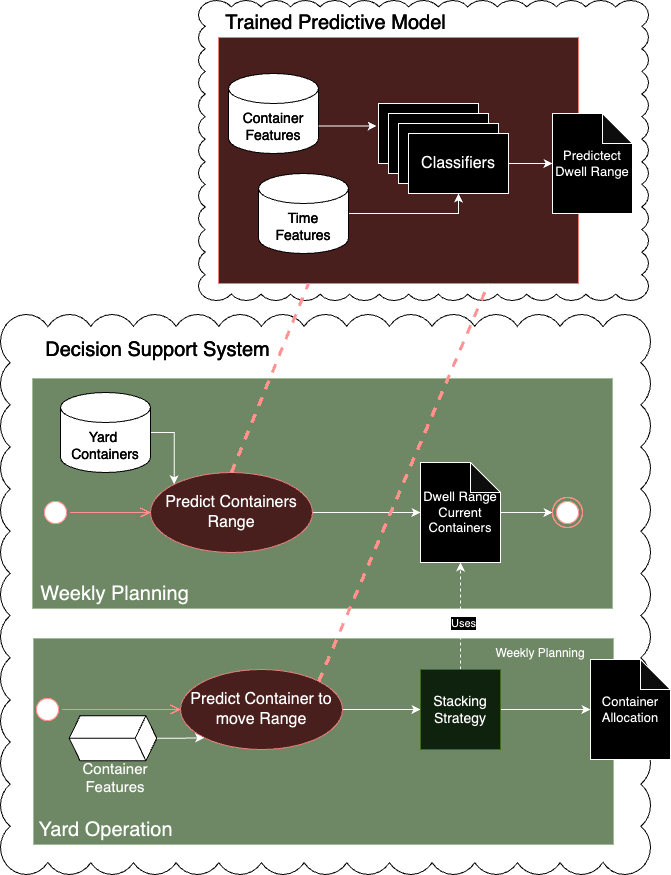
\includegraphics[width=1\textwidth]{images/DSS}
			\caption{DSS architecture using machine learning models}
			\label{fig:dds_architecture}
		\end{figure}
